% Orleans.StateMachineES Executive Overview
% Compile with: pdflatex statemachinees-executive-overview.tex (run twice for TOC)
\documentclass[11pt,a4paper]{article}

% ── Packages ──────────────────────────────────────────────────────────────────
\usepackage[utf8]{inputenc}
\usepackage[T1]{fontenc}
\usepackage{lmodern}
\usepackage[margin=2.4cm]{geometry}
\usepackage{graphicx}
\usepackage{xcolor}
\usepackage{titlesec}
\usepackage{enumitem}
\usepackage{booktabs}
\usepackage{tabularx}
\usepackage{multirow}
\usepackage{fancyhdr}
\usepackage{hyperref}
\usepackage{amssymb}
\usepackage{tcolorbox}
\usepackage{tikz}
\usepackage{pgfplots}
\pgfplotsset{compat=1.18}
\usetikzlibrary{arrows.meta, positioning, calc, shapes.geometric, backgrounds, fit}

% ── Colours ───────────────────────────────────────────────────────────────────
\definecolor{brand}{HTML}{512BD4}      % .NET Purple
\definecolor{accent}{HTML}{E85D04}     % Orange accent
\definecolor{highlight}{HTML}{0096C7}  % Bright cyan
\definecolor{success}{HTML}{2D936C}    % Green
\definecolor{lightbg}{HTML}{F4F6F9}    % Light background
\definecolor{midgray}{HTML}{6C757D}    % Muted text
\definecolor{orleans}{HTML}{3399FF}    % Orleans blue

% ── Heading styles ────────────────────────────────────────────────────────────
\titleformat{\section}
  {\Large\bfseries\color{brand}}
  {\thesection}{1em}{}[\vspace{-0.4em}\textcolor{accent}{\rule{\textwidth}{1.2pt}}]

\titleformat{\subsection}
  {\large\bfseries\color{brand}}
  {\thesubsection}{0.8em}{}

\titleformat{\subsubsection}
  {\normalsize\bfseries\color{accent}}
  {\thesubsubsection}{0.6em}{}

% ── Header / Footer ──────────────────────────────────────────────────────────
\pagestyle{fancy}
\fancyhf{}
\renewcommand{\headrulewidth}{0.4pt}
\fancyhead[L]{\small\textcolor{midgray}{Orleans.StateMachineES --- Executive Overview}}
\fancyhead[R]{\small\textcolor{midgray}{v1.1.0}}
\fancyfoot[C]{\small\textcolor{midgray}{\thepage}}

% ── Custom boxes ──────────────────────────────────────────────────────────────
\tcbset{
  keybox/.style={
    colback=lightbg, colframe=accent, boxrule=0.6pt,
    arc=3pt, left=8pt, right=8pt, top=6pt, bottom=6pt,
    fonttitle=\bfseries\color{brand}, title=#1
  },
  statbox/.style={
    colback=white, colframe=brand, boxrule=0.8pt,
    arc=4pt, left=6pt, right=6pt, top=4pt, bottom=4pt,
    width=0.30\textwidth
  }
}

% ── Hyperref setup ────────────────────────────────────────────────────────────
\hypersetup{
  colorlinks=true,
  linkcolor=brand,
  urlcolor=highlight,
  citecolor=brand,
  pdftitle={Orleans.StateMachineES -- Distributed State Machines for Microsoft Orleans},
  pdfauthor={Michael Ivertowski},
  pdfsubject={Executive Overview},
}

% ══════════════════════════════════════════════════════════════════════════════
\begin{document}

% ── Title page ────────────────────────────────────────────────────────────────
\begin{titlepage}
\begin{tikzpicture}[remember picture, overlay]
  % Background gradient bar
  \fill[brand] (current page.north west) rectangle
    ([yshift=-9cm]current page.north east);
  % Accent stripe
  \fill[accent] ([yshift=-9cm]current page.north west) rectangle
    ([yshift=-9.4cm]current page.north east);
  % Decorative dots
  \foreach \x in {0.5,1.0,...,5.0} {
    \foreach \y in {0.5,1.0,...,3.0} {
      \fill[white, opacity=0.04] ([xshift=\x cm, yshift=-\y cm]current page.north west)
        circle (1.5pt);
    }
  }
\end{tikzpicture}

\vspace*{1.5cm}
\begin{flushleft}
  {\fontsize{34}{40}\selectfont\bfseries\textcolor{white}{Orleans.StateMachineES}}\\[0.5em]
  {\fontsize{16}{20}\selectfont\textcolor{white!85}{Production-Ready Distributed State Machines for Microsoft Orleans}}\\[0.3em]
  {\large\textcolor{white!65}{Event Sourcing \textbullet{} Compile-Time Safety \textbullet{} Enterprise Resilience}}\\[0.3em]
  {\normalsize\textcolor{white!50}{.NET 9 \textbullet{} Orleans 9.1.2 \textbullet{} Stateless 5.17.0 \textbullet{} OpenTelemetry}}
\end{flushleft}

\vspace{5.5cm}

\begin{flushleft}
  \textcolor{midgray}{\large Executive Overview}\\[0.8em]
  {\Large\textcolor{brand}{\textbf{Version 1.1.0}}}\\[1.5em]
  \textcolor{midgray}{%
    A comprehensive framework for building distributed state machines\\
    with full event sourcing, hierarchical states, and enterprise-grade reliability.%
  }
\end{flushleft}

\vfill
\begin{flushleft}
  \textcolor{midgray}{\small
    Built with .NET \& Orleans \textbullet{} 3 NuGet Packages \textbullet{} 10 Roslyn Analyzers\\[4pt]
    Open-source (MIT License) \textbullet{} Published on NuGet.org\\[4pt]
    \textbf{Contact:} \href{mailto:michael.ivertowski@ch.ey.com}{michael.ivertowski@ch.ey.com}
  }
\end{flushleft}
\end{titlepage}

% ── Table of Contents ─────────────────────────────────────────────────────────
\tableofcontents
\newpage

% ══════════════════════════════════════════════════════════════════════════════
\section{Executive Summary}

Orleans.StateMachineES is a production-ready .NET library that integrates the
Stateless state machine library with Microsoft Orleans' actor framework. It
enables distributed state machine patterns in Orleans applications with full
event sourcing, hierarchical states, and enterprise-grade reliability features.
The library provides compile-time safety through 10 Roslyn analyzers and achieves
significant performance optimizations through intelligent caching.

\begin{tcolorbox}[keybox={Why Orleans.StateMachineES?}]
\begin{itemize}[leftmargin=1.2em, itemsep=3pt]
  \item \textbf{Event Sourcing} --- Complete state history with 30\%+ performance
        improvement through auto-confirmed events and snapshot support.
  \item \textbf{Compile-Time Safety} --- 10 Roslyn analyzers detect async anti-patterns,
        missing states, and design issues before runtime.
  \item \textbf{Enterprise Resilience} --- Circuit breakers, rate limiting, retry
        components, and distributed saga support with automatic compensation.
  \item \textbf{Production-Ready} --- OpenTelemetry tracing, health checks, state
        visualization, and comprehensive monitoring integration.
  \item \textbf{Performance Optimized} --- TriggerParameterCache delivers $\sim$100$\times$
        improvement for parameterized triggers with zero-allocation paths.
\end{itemize}
\end{tcolorbox}

\subsection{At a Glance}

\vspace{0.6em}
\begin{center}
\begin{tabular}{@{}c@{\hspace{1.8em}}c@{\hspace{1.8em}}c@{}}
% Row 1
\begin{tcolorbox}[statbox, width=4.8cm]
  \centering
  {\fontsize{26}{30}\selectfont\bfseries\textcolor{accent}{5,923}}\\[3pt]
  {\small transitions/sec (event sourced)}
\end{tcolorbox} &
\begin{tcolorbox}[statbox, width=4.8cm]
  \centering
  {\fontsize{26}{30}\selectfont\bfseries\textcolor{accent}{100$\times$}}\\[3pt]
  {\small trigger cache speedup}
\end{tcolorbox} &
\begin{tcolorbox}[statbox, width=4.8cm]
  \centering
  {\fontsize{26}{30}\selectfont\bfseries\textcolor{accent}{30\%+}}\\[3pt]
  {\small event sourcing gain}
\end{tcolorbox} \\[0.8em]
% Row 2
\begin{tcolorbox}[statbox, width=4.8cm]
  \centering
  {\fontsize{26}{30}\selectfont\bfseries\textcolor{accent}{10}}\\[3pt]
  {\small Roslyn analyzers}
\end{tcolorbox} &
\begin{tcolorbox}[statbox, width=4.8cm]
  \centering
  {\fontsize{26}{30}\selectfont\bfseries\textcolor{accent}{3}}\\[3pt]
  {\small NuGet packages}
\end{tcolorbox} &
\begin{tcolorbox}[statbox, width=4.8cm]
  \centering
  {\fontsize{26}{30}\selectfont\bfseries\textcolor{accent}{4}}\\[3pt]
  {\small example applications}
\end{tcolorbox}
\end{tabular}
\end{center}

% ══════════════════════════════════════════════════════════════════════════════
\newpage
\section{Core Abstractions}

\subsection{State Machine Grain Hierarchy}

Orleans.StateMachineES provides a layered grain hierarchy for different use cases,
from simple state machines to complex event-sourced workflows with hierarchical
states and distributed sagas.

\begin{table}[h!]
\centering
\renewcommand{\arraystretch}{1.25}
\begin{tabularx}{\textwidth}{>{\bfseries\color{brand}}l X}
\toprule
\textbf{Abstraction} & \textbf{Description} \\
\midrule
StateMachineGrain &
  Base grain wrapping Stateless with Orleans-compatible async methods,
  trigger parameter caching, and comprehensive state inspection APIs. \\
EventSourcedStateMachineGrain &
  Extends StateMachineGrain with JournaledGrain-based event sourcing,
  automatic snapshots, idempotency, and Orleans Streams integration. \\
TimerEnabledStateMachineGrain &
  Adds state-driven timeouts using Orleans Timers (short) and Reminders
  (durable), with repeating heartbeat patterns. \\
HierarchicalStateMachineGrain &
  Supports nested states with parent-child relationships, state path
  queries, and inheritance-based behavior. \\
VersionedStateMachineGrain &
  Semantic versioning, migration strategies (automatic, blue-green),
  shadow evaluation, and rollback support. \\
OrthogonalStateMachineGrain &
  Parallel independent state machines (regions) with cross-region
  synchronization and trigger mapping. \\
\bottomrule
\end{tabularx}
\end{table}

\subsection{State Machine Flow}

\begin{center}
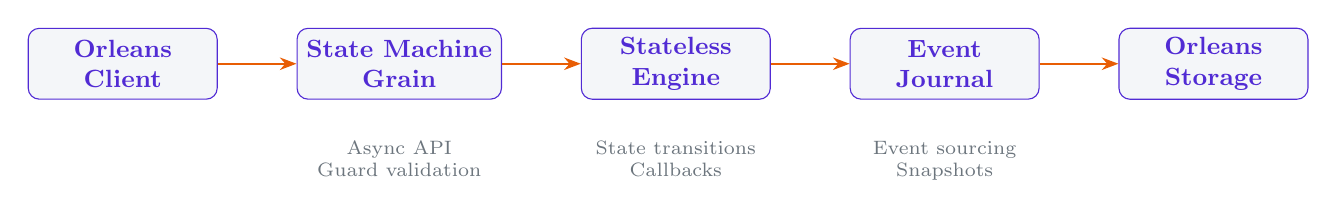
\begin{tikzpicture}[
  node distance=1.0cm,
  box/.style={draw=brand, fill=lightbg, rounded corners=4pt,
              minimum width=2.4cm, minimum height=0.9cm,
              font=\small\bfseries, text=brand, align=center},
  arr/.style={-{Stealth[length=6pt]}, thick, color=accent}
]
  \node[box] (client) {Orleans\\Client};
  \node[box, right=of client] (grain) {State Machine\\Grain};
  \node[box, right=of grain] (stateless) {Stateless\\Engine};
  \node[box, right=of stateless] (journal) {Event\\Journal};
  \node[box, right=of journal] (storage) {Orleans\\Storage};

  \draw[arr] (client) -- (grain);
  \draw[arr] (grain) -- (stateless);
  \draw[arr] (stateless) -- (journal);
  \draw[arr] (journal) -- (storage);

  \node[below=0.4cm of grain, font=\scriptsize\color{midgray}, align=center]
    {Async API\\Guard validation};
  \node[below=0.4cm of stateless, font=\scriptsize\color{midgray}, align=center]
    {State transitions\\Callbacks};
  \node[below=0.4cm of journal, font=\scriptsize\color{midgray}, align=center]
    {Event sourcing\\Snapshots};
\end{tikzpicture}
\end{center}

% ══════════════════════════════════════════════════════════════════════════════
\newpage
\section{Compile-Time Safety}

\subsection{Roslyn Analyzer Suite}

Orleans.StateMachineES includes 10 comprehensive Roslyn analyzers that detect
anti-patterns at compile time, preventing runtime issues before deployment.

\begin{table}[h!]
\centering
\renewcommand{\arraystretch}{1.2}
\begin{tabularx}{\textwidth}{>{\ttfamily\color{brand}}l l X}
\toprule
\textbf{ID} & \textbf{Severity} & \textbf{Description} \\
\midrule
OSMES001 & Warning & Async lambda in state callback (OnEntry, OnExit) \\
OSMES002 & Error & FireAsync called within state callback \\
OSMES003 & Warning & Missing initial state configuration \\
OSMES004 & Warning & Unreachable state detected \\
OSMES005 & Info & Multiple entry callbacks on same state \\
OSMES006 & Warning & State has no trigger handlers \\
OSMES007 & Warning & Circular state transitions with no exit path \\
OSMES008 & Warning & Guard condition complexity too high ($> 10$) \\
OSMES009 & Error & State machine missing initial state assignment \\
OSMES010 & Warning & Invalid enum value cast (unsafe numeric cast) \\
\bottomrule
\end{tabularx}
\end{table}

\subsection{Async Safety Protection}

The underlying Stateless library does \textbf{not} support async operations in
state callbacks. Orleans.StateMachineES provides both compile-time and runtime
protection:

\begin{tcolorbox}[keybox={Protection Layers}]
\begin{itemize}[leftmargin=1.2em, itemsep=3pt]
  \item \textbf{OSMES001} --- Warns when async lambdas are used in OnEntry/OnExit
  \item \textbf{OSMES002} --- Errors when FireAsync is called within callbacks
  \item \textbf{Runtime Validation} --- Thread-local tracking prevents nested FireAsync
  \item \textbf{Clear Error Messages} --- Actionable guidance for correct patterns
\end{itemize}
\end{tcolorbox}

% ══════════════════════════════════════════════════════════════════════════════
\newpage
\section{Key Features}

\subsection{Event Sourcing}

Event sourcing provides complete audit trails with automatic state replay:

\begin{table}[h!]
\centering
\renewcommand{\arraystretch}{1.2}
\begin{tabularx}{\textwidth}{>{\bfseries\color{brand}}l X}
\toprule
\textbf{Feature} & \textbf{Details} \\
\midrule
Auto-Confirmed Events &
  30\%+ performance improvement with \texttt{AutoConfirmEvents = true},
  achieving 5,923 transitions/sec (0.17ms latency). \\
Snapshots &
  Configurable snapshot intervals for large event histories, with automatic
  state reconstruction on grain activation. \\
Idempotency &
  Built-in deduplication with LRU cache prevents duplicate command processing
  in distributed scenarios. \\
Stream Integration &
  Publish state transitions to Orleans Streams for real-time event processing
  and external system notifications. \\
Correlation Tracking &
  Track related events across distributed systems with correlation IDs
  propagated through sagas and workflows. \\
\bottomrule
\end{tabularx}
\end{table}

\subsection{Production Enhancements (v1.1.0)}

\begin{table}[h!]
\centering
\renewcommand{\arraystretch}{1.2}
\begin{tabularx}{\textwidth}{>{\bfseries\color{brand}}l X}
\toprule
\textbf{Component} & \textbf{Capabilities} \\
\midrule
Rate Limiting &
  Token bucket algorithm with configurable burst capacity, sliding/fixed
  windows, and real-time utilization statistics. \\
Batch Operations &
  Parallel execution API with configurable parallelism, exponential backoff
  retry, and progress tracking. \\
Event Schema Evolution &
  Automatic event upcasting with BFS-based version chain discovery for
  multi-step event upgrades. \\
Persistence Abstraction &
  Provider-agnostic IEventStore, ISnapshotStore, IStateMachinePersistence
  with in-memory and provider options (CosmosDB, PostgreSQL, MongoDB). \\
State Machine Templates &
  Reusable patterns: ApprovalWorkflow, OrderProcessing, RetryableOperation
  with configurable parameters. \\
State History Queries &
  Fluent LINQ-style API for temporal queries with GroupByState, GroupByTrigger,
  GroupByTime analytics. \\
\bottomrule
\end{tabularx}
\end{table}

% ══════════════════════════════════════════════════════════════════════════════
\newpage
\section{Enterprise Resilience}

\subsection{Circuit Breaker Pattern}

Production-ready resilience component with three-state management:

\begin{center}
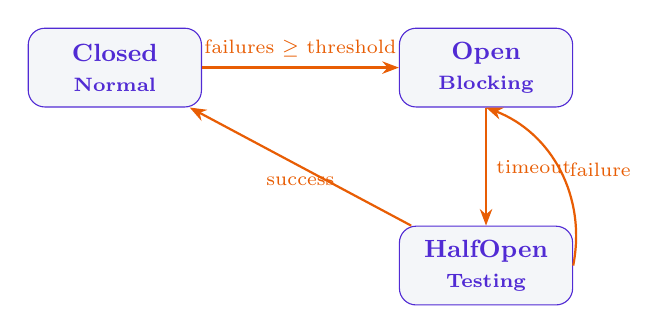
\begin{tikzpicture}[
  node distance=2.5cm,
  state/.style={draw=brand, fill=lightbg, rounded corners=6pt,
                minimum width=2.2cm, minimum height=1cm,
                font=\small\bfseries, text=brand, align=center},
  arr/.style={-{Stealth[length=6pt]}, thick, color=accent}
]
  \node[state] (closed) {Closed\\{\scriptsize Normal}};
  \node[state, right=of closed] (open) {Open\\{\scriptsize Blocking}};
  \node[state, below=1.5cm of open] (half) {HalfOpen\\{\scriptsize Testing}};

  \draw[arr] (closed) -- node[above, font=\scriptsize\color{midgray}] {failures $\geq$ threshold} (open);
  \draw[arr] (open) -- node[right, font=\scriptsize\color{midgray}] {timeout} (half);
  \draw[arr] (half) -- node[below, font=\scriptsize\color{midgray}] {success} (closed);
  \draw[arr] (half.east) to[bend right=40] node[right, font=\scriptsize\color{midgray}] {failure} (open.south);
\end{tikzpicture}
\end{center}

\begin{table}[h!]
\centering
\renewcommand{\arraystretch}{1.2}
\begin{tabularx}{\textwidth}{>{\bfseries\color{brand}}l X}
\toprule
\textbf{Configuration} & \textbf{Purpose} \\
\midrule
FailureThreshold & Number of consecutive failures before opening (default: 5) \\
SuccessThreshold & Successes needed in HalfOpen to close (default: 2) \\
OpenDuration & Time before testing recovery (default: 30s) \\
MonitoredTriggers & Specific triggers to protect with circuit breaker \\
ThrowWhenOpen & Throw exception or return false when circuit is open \\
\bottomrule
\end{tabularx}
\end{table}

\subsection{Distributed Sagas}

Orchestration-based multi-grain workflows with automatic compensation:

\begin{tcolorbox}[keybox={Saga Features}]
\begin{itemize}[leftmargin=1.2em, itemsep=3pt]
  \item \textbf{Step Orchestration} --- Central saga coordinator manages business process
  \item \textbf{Automatic Compensation} --- Failed steps trigger rollback in reverse order
  \item \textbf{Retry Logic} --- Exponential backoff for technical failures
  \item \textbf{Business vs Technical Errors} --- Different handling strategies
  \item \textbf{Timeout Management} --- Per-step timeouts with graceful degradation
  \item \textbf{Full Audit Trail} --- Event-sourced saga execution history
\end{itemize}
\end{tcolorbox}

% ══════════════════════════════════════════════════════════════════════════════
\newpage
\section{Architecture}

\subsection{Project Structure}

\begin{center}
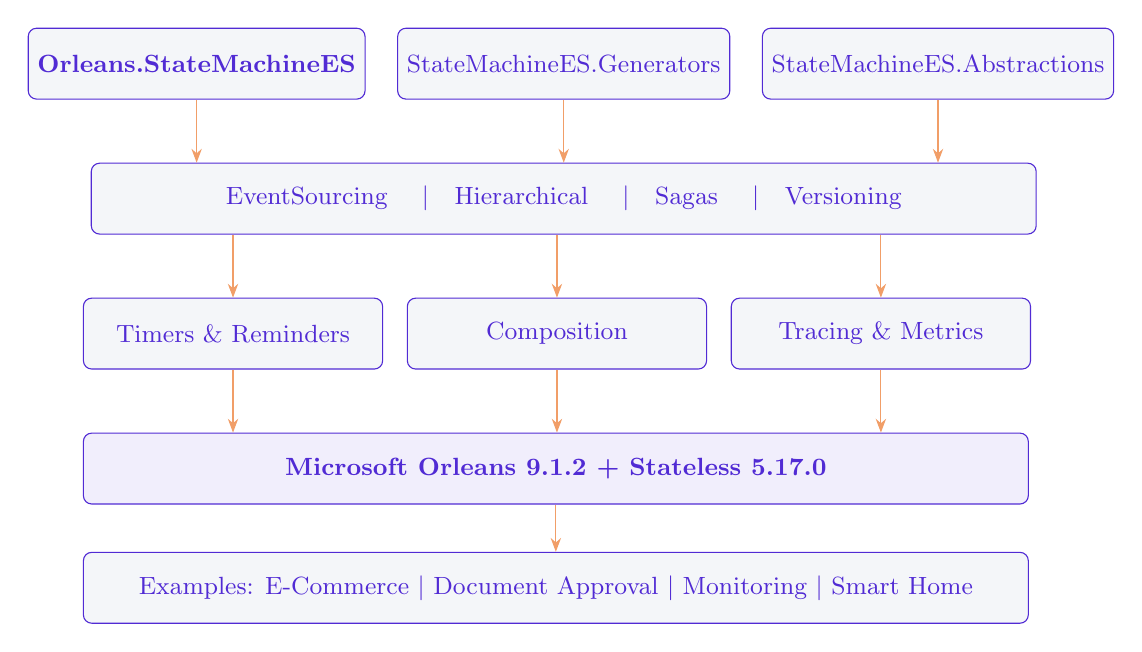
\begin{tikzpicture}[
  node distance=0.5cm,
  layer/.style={draw=brand, fill=lightbg, rounded corners=3pt,
                minimum height=0.9cm, font=\small, text=brand, align=center},
  arr/.style={-{Stealth[length=5pt]}, color=accent!60}
]
  % Top layer - Main packages
  \node[layer, minimum width=4.0cm] (main) {\textbf{Orleans.StateMachineES}};
  \node[layer, minimum width=4.0cm, right=0.4cm of main] (gen) {StateMachineES.Generators};
  \node[layer, minimum width=3.0cm, right=0.4cm of gen] (abs) {StateMachineES.Abstractions};

  % Feature layer
  \node[layer, minimum width=12.0cm, below=0.8cm of gen] (features)
    {EventSourcing \quad\textbar\quad Hierarchical \quad\textbar\quad Sagas \quad\textbar\quad Versioning};

  % Component layer
  \node[layer, minimum width=3.8cm, below=0.8cm of features.south west,
        anchor=north west, xshift=-0.1cm] (timers) {Timers \& Reminders};
  \node[layer, minimum width=3.8cm, right=0.3cm of timers] (compose) {Composition};
  \node[layer, minimum width=3.8cm, right=0.3cm of compose] (observe) {Tracing \& Metrics};

  % Infrastructure
  \node[layer, minimum width=12.0cm, below=0.8cm of timers.south west,
        anchor=north west, fill=brand!8]
    (infra) {\textbf{Microsoft Orleans 9.1.2 + Stateless 5.17.0}};

  % Examples
  \node[layer, minimum width=12.0cm, below=0.6cm of infra]
    (examples) {Examples: E-Commerce \textbar{} Document Approval \textbar{} Monitoring \textbar{} Smart Home};

  % Arrows
  \draw[arr] (main.south) -- (main.south |- features.north);
  \draw[arr] (gen.south) -- (features.north);
  \draw[arr] (abs.south) -- (abs.south |- features.north);

  \draw[arr] (features.south -| timers) -- (timers.north);
  \draw[arr] (features.south -| compose) -- (compose.north);
  \draw[arr] (features.south -| observe) -- (observe.north);

  \draw[arr] (timers.south) -- (timers.south |- infra.north);
  \draw[arr] (compose.south) -- (compose.south |- infra.north);
  \draw[arr] (observe.south) -- (observe.south |- infra.north);
  \draw[arr] (infra.south) -- (examples.north);
\end{tikzpicture}
\end{center}

\subsection{NuGet Packages}

\begin{table}[h!]
\centering
\renewcommand{\arraystretch}{1.2}
\begin{tabularx}{\textwidth}{>{\bfseries\color{brand}}l l X}
\toprule
\textbf{Package} & \textbf{Version} & \textbf{Contents} \\
\midrule
Orleans.StateMachineES &
  1.1.0 &
  Main library with all grain implementations, event sourcing, sagas,
  versioning, visualization, and enterprise components. \\
Orleans.StateMachineES.Abstractions &
  1.1.0 &
  Core interfaces (IStateMachineGrain), models, and shared abstractions
  for extending the library. \\
Orleans.StateMachineES.Generators &
  1.1.0 &
  Roslyn source generator for YAML/JSON specifications and 10 compile-time
  analyzers with full XML documentation. \\
\bottomrule
\end{tabularx}
\end{table}

% ══════════════════════════════════════════════════════════════════════════════
\newpage
\section{Observability \& Monitoring}

\subsection{OpenTelemetry Integration}

Built-in distributed tracing and metrics for production visibility:

\begin{table}[h!]
\centering
\renewcommand{\arraystretch}{1.2}
\begin{tabularx}{\textwidth}{>{\bfseries\color{brand}}l X}
\toprule
\textbf{Capability} & \textbf{Details} \\
\midrule
Activity Tracing &
  Automatic spans for state transitions with grain type, ID, states, and
  trigger information. Supports Jaeger, Zipkin, OTLP exporters. \\
Metrics Collection &
  Counters and histograms: transitions\_total, transition\_duration,
  active\_grains, trigger\_errors\_total, saga\_executions\_total. \\
TracingHelper &
  Utility class for custom operation tracing with correlation context
  and saga step tracking. \\
Health Checks &
  ASP.NET Core health check integration with custom providers for
  state machine grain health monitoring. \\
\bottomrule
\end{tabularx}
\end{table}

\subsection{State Machine Visualization}

\begin{table}[h!]
\centering
\renewcommand{\arraystretch}{1.2}
\begin{tabularx}{\textwidth}{>{\bfseries\color{brand}}l X}
\toprule
\textbf{Feature} & \textbf{Capabilities} \\
\midrule
Export Formats &
  DOT (Graphviz), Mermaid (GitHub markdown), PlantUML, JSON, XML,
  and interactive HTML with real-time updates. \\
Structural Analysis &
  Cyclomatic complexity, state count, max depth, connectivity index,
  unreachable state detection, and design recommendations. \\
Batch Visualization &
  Analyze multiple grain types simultaneously with comparative
  statistics and generated reports. \\
Web Dashboard &
  Interactive HTML visualization with Vis.js, live state tracking,
  transition history, and performance metrics. \\
\bottomrule
\end{tabularx}
\end{table}

% ══════════════════════════════════════════════════════════════════════════════
\section{Use Cases}

\begin{tcolorbox}[keybox={Primary Use Cases}]
\begin{description}[leftmargin=1em, labelwidth=1em, font=\color{brand}\bfseries]
  \item[$\blacktriangleright$] \textbf{E-Commerce Workflows} ---
    Order processing with payment timeouts, shipping state tracking,
    and complete audit trails through event sourcing.

  \item[$\blacktriangleright$] \textbf{Document Approval} ---
    Multi-level approval workflows with hierarchical states, parallel
    review processes, and automatic escalation.

  \item[$\blacktriangleright$] \textbf{IoT Device Control} ---
    Smart home automation with orthogonal regions for independent
    subsystems (security, climate, energy) and cross-region sync.

  \item[$\blacktriangleright$] \textbf{Financial Processing} ---
    Invoice processing sagas with automatic compensation, audit
    compliance, and distributed transaction coordination.

  \item[$\blacktriangleright$] \textbf{Microservice Orchestration} ---
    Long-running business processes with durable reminders, version
    migration, and graceful degradation.

  \item[$\blacktriangleright$] \textbf{Compliance \& Audit} ---
    Complete state history with temporal queries, event replay for
    debugging, and regulatory reporting.
\end{description}
\end{tcolorbox}

% ══════════════════════════════════════════════════════════════════════════════
\newpage
\section{Getting Started}

\subsection{Quick Start (NuGet)}

\begin{tcolorbox}[colback=brand!3, colframe=brand!40, boxrule=0.5pt, arc=3pt,
                   left=8pt, right=8pt, top=6pt, bottom=6pt]
\ttfamily\small
\# Add packages via CLI\\
dotnet add package Orleans.StateMachineES\\
dotnet add package Orleans.StateMachineES.Generators\\[6pt]
\# Or in .csproj\\
<PackageReference Include="Orleans.StateMachineES" Version="1.1.0" />\\
<PackageReference Include="Orleans.StateMachineES.Generators" Version="1.1.0" />
\end{tcolorbox}

\subsection{Basic State Machine Grain}

\begin{tcolorbox}[colback=brand!3, colframe=brand!40, boxrule=0.5pt, arc=3pt,
                   left=8pt, right=8pt, top=6pt, bottom=6pt]
\ttfamily\small
public class DoorGrain : StateMachineGrain<DoorState, DoorTrigger>, IDoorGrain\\
\{\\
\hspace{1em}protected override StateMachine<DoorState, DoorTrigger> BuildStateMachine()\\
\hspace{1em}\{\\
\hspace{2em}var machine = new StateMachine<DoorState, DoorTrigger>(DoorState.Closed);\\[4pt]
\hspace{2em}machine.Configure(DoorState.Closed)\\
\hspace{3em}.Permit(DoorTrigger.Open, DoorState.Open)\\
\hspace{3em}.Permit(DoorTrigger.Lock, DoorState.Locked);\\[4pt]
\hspace{2em}machine.Configure(DoorState.Open)\\
\hspace{3em}.Permit(DoorTrigger.Close, DoorState.Closed);\\[4pt]
\hspace{2em}return machine;\\
\hspace{1em}\}\\
\}
\end{tcolorbox}

\subsection{Event-Sourced State Machine}

\begin{tcolorbox}[colback=brand!3, colframe=brand!40, boxrule=0.5pt, arc=3pt,
                   left=8pt, right=8pt, top=6pt, bottom=6pt]
\ttfamily\small
public class OrderGrain : EventSourcedStateMachineGrain<OrderState, OrderTrigger, OrderState>\\
\{\\
\hspace{1em}protected override void ConfigureEventSourcing(EventSourcingOptions options)\\
\hspace{1em}\{\\
\hspace{2em}options.AutoConfirmEvents = true;  // Critical for performance!\\
\hspace{2em}options.EnableSnapshots = true;\\
\hspace{2em}options.SnapshotInterval = 100;\\
\hspace{1em}\}\\
\}
\end{tcolorbox}

% ══════════════════════════════════════════════════════════════════════════════
\vspace{1.5em}
\begin{tcolorbox}[keybox={Links \& Resources}]
\renewcommand{\arraystretch}{1.4}
\begin{tabularx}{\textwidth}{>{\bfseries\color{brand}}l X}
  Repository &
    \url{https://github.com/mivertowski/Orleans.StateMachineES} \\
  Documentation &
    \url{https://mivertowski.github.io/Orleans.StateMachineES/} \\
  NuGet &
    \url{https://www.nuget.org/packages/Orleans.StateMachineES/} \\
  API Reference &
    \url{https://mivertowski.github.io/Orleans.StateMachineES/api/} \\
  Examples &
    See \texttt{examples/} directory for E-Commerce, Document Approval,\\
    & Monitoring Dashboard, and Smart Home applications \\
\end{tabularx}
\end{tcolorbox}

\vfill
\begin{center}
\textcolor{midgray}{\rule{0.5\textwidth}{0.4pt}}\\[0.8em]
{\small\textcolor{midgray}{%
  Orleans.StateMachineES v1.1.0 \textbullet{}
  Open-source (MIT License) \textbullet{}
  Published on NuGet.org%
}}\\[4pt]
{\small\textcolor{midgray}{%
  \textbf{Author:} Michael Ivertowski \textbullet{}
  \textbf{Contact:} \href{mailto:michael.ivertowski@ch.ey.com}{michael.ivertowski@ch.ey.com}%
}}
\end{center}

\end{document}
